\documentclass{beamer}
\usepackage{hyperref}
\usepackage[T1]{fontenc}
\usepackage{cite}
\usepackage{relsize}
\usepackage{animate}


\usefonttheme[onlymath]{serif}
%C++ symbol
\newcommand{\Rplus}{\protect\hspace{-.1em}\protect\raisebox{.35ex}{\smaller{\smaller\textbf{+}}}}
\newcommand{\Cpp}{\mbox{C\Rplus\Rplus}\hspace{3pt}}
%Scientific notation
\newcommand{\expnumber}[2]{{#1}\mathrm{e}{#2}}

\usepackage{latexsym,amsmath,xcolor,multicol,booktabs,calligra}
\usepackage{graphicx,tikz,listings,stackengine}
\usetikzlibrary{matrix, positioning}
\setbeamertemplate{bibliography item}[text]

\author{Rafael De Luna Loredo}
\title{Estructuras de Datos y Algoritmos}
\subtitle{Programación en Python y \Cpp}
\institute{Facultad de Ciencias, UASLP}
\date{}
\usepackage{NJFU}

% defs
\def\cmd#1{\texttt{\color{red}\footnotesize $\backslash$#1}}
\def\env#1{\texttt{\color{blue}\footnotesize #1}}
\definecolor{deepblue}{rgb}{0,0,0.5}
\definecolor{deepred}{rgb}{0.6,0,0}
\definecolor{deepgreen}{rgb}{0,0.5,0}
\definecolor{halfgray}{gray}{0.55}


\lstset{
    basicstyle=\ttfamily\small,
    keywordstyle=\bfseries\color{deepblue},
    emphstyle=\ttfamily\color{deepred},    
    stringstyle=\color{deepgreen},
    numbers=left,
    numberstyle=\small\color{halfgray},
    rulesepcolor=\color{red!20!green!20!blue!20},
    frame=shadowbox
}

\begin{document}

\AtBeginSubsection[]
{
  \begin{frame}
  \begin{multicols}{3}
    \tableofcontents[currentsection,subsectionstyle=show/shaded/hide,subsubsectionstyle=show/shaded/hide]
   \end{multicols}
  \end{frame}
}
\AtBeginSubsubsection[]{
	\begin{frame}
		\begin{multicols}{3}
			\tableofcontents[currentsection,subsectionstyle=show/shaded/hide,subsubsectionstyle=show/shaded/hide]
		\end{multicols}
	\end{frame}
}

\AtBeginSection[]
{
	\begin{frame}
		\begin{multicols*}{3}
			\tableofcontents[currentsection,subsectionstyle=show/shaded/hide,subsubsectionstyle=show/shaded/hide]
		\end{multicols*}
	\end{frame}
}

\begin{frame}
    \titlepage
    \begin{figure}[htpb]
        \begin{center}
            
\includegraphics[width=0.2\linewidth]{fig/logo.png}
        \end{center}
    \end{figure}
\end{frame}

\begin{frame}{Indice}
    \begin{multicols*}{3}
        \tableofcontents[sectionstyle=show,subsectionstyle=show/shaded/hide,subsubsectionstyle=show/shaded/hide]
    \end{multicols*}
\end{frame}

\section{Introducción}

\begin{frame}{\textquestiondown Qué es un algoritmo?}
Es una serie de pasos a seguir para solucionar un problema.\newline
Pero no solo eso, incluso en nuestra vida diaria usamos algoritmos sin saberlo, por ejemplo al ponernos los zapatos o vestirnos seguimos una serie de pasos para llegar a un resultado final
\end{frame}

\begin{frame}{\textquestiondown Como programar algoritmos?}
Antes de empezar a tirar código hay que hacernos unas cu\'antas preguntas
    \begin{itemize}
        \item \textquestiondown sigue una serie de pasos?
        \item \textquestiondown son consecutivos?
        \item \textquestiondown que resultados puedo esperar?
    \end{itemize}
\end{frame}

\begin{frame}{\textquestiondown Que lenguajes de programaci\'on usar?}
Podemos hacer uso de cualquier lenguaje, todo depender\'a de que tan c\'omodos nos sintamos con el lenguaje
que vayamos a usar o estemos utilizando.\newline
En este curso veremos los ejemplos en Python y \Cpp, \Cpp por ser el m\'as utilizado en programaci\'on competitiva y Python por su s\'intaxis sencilla y su amplia utilizaci\'on en la industria.
\end{frame}

\subsection{Conceptos B\'asicos}

\subsubsection{Bibliotecas, cabeceras, espacio de nombres}

\begin{frame}{Cabeceras}
        Son archivos que contienen las declaraciones de funciones y/o clases por lo que suelen tener c\'odigo
\end{frame}

\begin{frame}{Bibliotecas}
    Una biblioteca o libreria podriamos considerarla una colecci\'on de cabeceras, adem\'as de cabeceras incluye archivos de enlazado din\'amico o est\'atico.
\end{frame}

\begin{frame}{Espacio de nombres}
	Es un contenedor donde existen una o m\'as identificadores para clases, funciones \'o met\'odos contenidos en las cabeceras.
\end{frame}


\subsection{Tipos de Datos}

\subsubsection{N\'umericos}

\begin{frame}{Enteros}
    \begin{itemize}
        \item No aceptan decimales
        \item Pueden ser negativos o positivos
        \item En \Cpp ocupan 4 bytes de memoria y un valor m\'aximo de $\pm 2147483647$ 
        \item En Python var\'ia el tamño en memoria pero puede ser desde 28 bytes hasta 408 bytes o m\'as
    \end{itemize}
\end{frame}

\begin{frame}{Reales}
    \begin{itemize}
        \item Aceptan decimales
        \item Pueden ser negativos o positivos
        \item En \Cpp  ocupan 4 bytes de memoria y valores entre $\expnumber{1.17549}{-38}$ y $\expnumber{3.40282}{+38}$ 
        \item En Python var\'ia el tamaño en memoria pero puede ser desde 24 bytes hasta 408 bytes o m\'asp
    \end{itemize}
\end{frame}

\begin{frame}{Reales de doble precisi\'on}
    \begin{itemize}
        \item Aceptan decimales
        \item Pueden ser negativos o positivos
        \item En \Cpp  ocupan 8 bytes de memoria y valores entre $\expnumber{2.22507}{-308}$ y $\expnumber{1.79769}{+308}$ 
        \item En Python el tipo float hace una implementaci\'on a bajo nivel del tipo \textbf{double} de C.
    \end{itemize}
\end{frame}

\subsubsection{Caracteres}

\begin{frame}{Caracter}
    \begin{itemize}
        \item Representan letras, simbolos o caracteres
        \item En \Cpp  ocupan 1 byte de memoria y valores  de $\pm 127$ 
        \item En Python como tal no existe.
    \end{itemize}
\end{frame}

\begin{frame}{Cadena de caracteres}
    \begin{itemize}
        \item Representan letras, simbolos, caracteres y/o palabras
        \item Tanto en \Cpp como en Python el tamaño var\'ia seg\'un el tamaño de la cadena
        \item En el caso de \Cpp existen dos tipos, un arreglo de tipo \textbf{char} y el tipo \textbf{str} a tr\'aves de la biblioteca \textbf{cstring}
    \end{itemize}
\end{frame}

\subsubsection{Lógicos}

\begin{frame}{Booleanos}
    \begin{itemize}
        \item Representan solamente \textbf{True} o \textbf{False}, \textbf{1} o \textbf{0}
        \item Ocupan 1 byte de almacenamiento, por lo que se desperdicia mucho espacio de memoria
    \end{itemize}
\end{frame}


\subsubsection{Contenedores y colecciones}

\begin{frame}{Diccionarios}
    \begin{itemize}
        \item Se componen de una llave o clave y un valor
        \item Son elementos ordenados
        \item Pueden existir m\'ultiples llaves
        \item Las llaves no se pueden repetir
        \item En \Cpp se llaman mapas, para usarlos hay que importar la cabecera \textit{map}
    \end{itemize}
\end{frame}

\begin{frame}{Listas}
    \begin{itemize}
        \item Son una secuencia de elementos
        \item En Python pueden contener m\'ultiples tipos de datos
        \item Para usarlos en \Cpp hay que importar la cabecera \textit{list}
    \end{itemize}
\end{frame}

\begin{frame}{Tuplas}
    \begin{itemize}
        \item Son una secuencia de elementos
        \item Pueden contener m\'ultiples tipos de datos
        \item En Python son inmutables, es decir no se pueden modificar o eliminar elementos
        \item Para usarlos en \Cpp hay que importar la cabecera \textit{tuple}
    \end{itemize}
\end{frame}

\begin{frame}{Conjuntos}
    \begin{itemize}
        \item Son una secuencia de elementos no repetidos
        \item Hacen alusi\'on a la definici\'on matem\'atica de conjuntos
        \item En \Cpp existen dos tipos, ordenados y no ordenados
        \item Para usarlos en \Cpp hay que importar las cabeceras \textit{set} y \textit{unordered\_set} respectivamente\nocite{BHASIN,BJARNE1,BJARNE2,CAIRO,CPP,DEITEL,DOWNEY,JAWORSKI,KENN,lAAKMANN,MATTHES,RAMALHO,SED}
    \end{itemize}
\textbf{}\end{frame}

\section{Operaciones}

\begin{frame}{Operaciones Matem\'aticas}
    \begin{itemize}
        \item Tienen orden de precedencia, siendo el mismo que conocemos en matem\'aticas
        \item Van de izquierda a derecha
        \item Se realizan en pares
        \item Se pueden realizar entre diferentes tipos, todo dependera de si se guardan o no en una variable
        \item Son las mismas que en matem\'aticas, suma, resta, multiplicaci\'on, divisi\'on y m\'odulo o residuo
        \item Para uso de funciones mas avanzadas habrá que hacer uso de cabeceras o bibliotecas creadas para dicho prop\'osito
    \end{itemize}
\end{frame}

\begin{frame}{Operaciones L\'ogicas}
    \begin{itemize}
        \item Devuelven un valor booleano
        \item Van de izquierda a derecha
        \item Se realizan en pares
        \item Son algunas que ya conocemos en matem\'aticas, mayor que, menor que, igual a, diferente de, menor o igual,mayor o igual, conjunc\'on y disyunci\'on
        \item La conjunci\'on y disyunci\'on dependen de las otras
    \end{itemize}
\end{frame}

\section{Condicionales}

\begin{frame}{Introducci\'on}
    \begin{itemize}
        \item Son un tipo de estructura
        \item Nos ayudan a tener control seg\'un valores o resultados esperados
        \item Eval\'uan operaciones l\'ogicas
        \item Pueden contener o concatenar m\'ultiples estructuras
    \end{itemize}
\end{frame}

\subsection{if else elif}

\begin{frame}{if}
    Nos ayuda a evaluar si una condici\'on existe, en caso de que se cumpla, se ejecuta el c\'odigo que contiene
\end{frame}

\begin{frame}{else}
    Es la contraparte de \textbf{if}, en caso de que la condici\'on de \textbf{if} no se cumpla, ejecuta el c\'odigo que contiene
\end{frame}

\begin{frame}{elif}
    Es una combinaci\'on de \textbf{else} con \textbf{if}, hace una segunda evaluaci\'on de otro posible resultado esperado
\end{frame}

\subsection{Switch}

\begin{frame}{Switch}
    \begin{itemize}
        \item En Python no existe pero se puede hacer con diccionarios o ecandenando m\'ultiples \textbf{if else}
        \item Es una estructura que eval\'ua m\'ultiples casos posibles en base al posible valor de una variable
        \item Tambi\'en puede contener otras estructuras
    \end{itemize}
\end{frame}

\subsection{Operador ternario}

\begin{frame}{Operador ternario}
    \begin{itemize}
        \item El funcionamiento es como el de un \textbf{if}, en Python de hecho es un \textbf{if}
        \item Sirve para comparaciones simples, donde no necesitamos ejecutar mucho c\'odigo
    \end{itemize}
\end{frame}

\section{Ciclos}

\begin{frame}{Introducci\'on}
    \begin{itemize}
        \item Son un tipo de estructura
        \item Nos ayudan a ejecutar un c\'odigo m\'ultiples veces
        \item Ayudan a reducir c\'odigo
    \end{itemize}
\end{frame}

\begin{frame}{for}
    \begin{itemize}
        \item Se define un contador
        \item El contador cambia sin necesidad de declarar dicho cambio
        \item Hay que definir un tope o l\'imite
        \item Hay que definir como avanza el contador
    \end{itemize}
\end{frame}


\begin{frame}{while}
    \begin{itemize}
        \item Se ejecuta mientras dada una condici\'on, dicha condici\'on exista o se cumpla
        \item No se define un l\'imite, mientras la condici\'on exista, se seguir\'a ejecutando 
        \item Necesitamos crear una manera de salir, por si la condici\'on sigue existiendo
        \item Podr\'ia no ejecutarse si la conidici\'on no existe antes de hacer la evaluaci\'on
    \end{itemize}
\end{frame}

\begin{frame}{do while}
    \begin{itemize}
            \item Es muy parecido a \textbf{while} con la diferencia de que primero ejecuta y despu\'es comprueba si dicha condici\'on existe
            \item No se define un l\'imite, mientras la condici\'on exista, se seguir\'a ejecutando
            \item Necesitamos crear una manera de salir, por si la condici\'on sigue existiendo
            \item Se ejecuta al menos una vez
            \item En Python no existe
        \end{itemize}
\end{frame}

\section{Arreglos  y Matrices}

\subsection{Arreglos}
\begin{frame}{Introducci\'on}
    \begin{itemize}
            \item Son de un solo tipo
            \item Puede contener m\'ultiples valores
            \item Es unidimensional
            \item Su espacio en memoria var\'ia seg\'un el tipo de dato y los valores que pueda tener
            \item En Python como tal no existen,  se usan las listas en su lugar
            \item El \'indice siempre empieza en cero, puede variar en algunos lenguajes, pero suele ser una regla general
        \end{itemize}
\end{frame}

\subsubsection{M\'etodos}

\begin{frame}{Almacenamiento en memoria}
	\begin{itemize}
		\item El valor nos \'indica el contenido del arreglo en determinada posici\'on
		\item El \'indice nos indica la posici\'on en el arreglo
		\item La direcci\'on de memoria donde se encuentra almacenado dicho valor	
	\end{itemize}
	\centering
    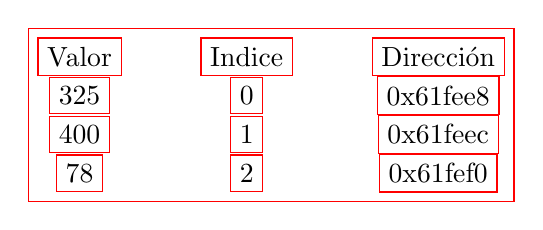
\begin{tikzpicture}[ampersand replacement=\&,every node/.style={draw}]
    	\matrix [draw=red,column sep=1cm]
    	{
    		\node {Valor}; \& \node {Indice}; \& \node{Direcci\'on}; \\
    		\node {325}; \& \node{0}; \& \node {0x61fee8}; \\
    		\node {400}; \& \node{1}; \& \node {0x61feec}; \\
    		\node {78}; \& \node{2}; \& \node {0x61fef0}; \\
    	};
    \end{tikzpicture}
\end{frame}


\begin{frame}{Insertar en \Cpp}
	\begin{itemize}
		\item Hay que conocer el \'indice donde queremos el valor
		\item No es necesario insertarlos en orden
		\item No se puede tener un \'indice mayor al tamaño del arreglo
	\end{itemize}
	\centering
	\animategraphics[autoplay,loop,width=4cm]{20}{animaciones/array/insertion/insertion-}{0}{216}
\end{frame}

\begin{frame}{Insertar en Python}
	\begin{itemize}
		\item Las listas en Python tienen un m\'etodo para agregar valores
		\item No es necesario conocer el \'indice
		\item No es necesario conocer el tamaño 
	\end{itemize}
\end{frame}

\begin{frame}{Modificar}
	\begin{itemize}
		\item Hay que conocer el \'indice
		\item No se puede tener un \'indice mayor al tamaño del arreglo
	\end{itemize}
\end{frame}

\begin{frame}{Eliminar}
	\begin{itemize}
		\item En \Cpp no se puede eliminar un elemento de un arreglo, solo se ignora el \'indice 
		\item En Python existen 3 m\'etodos \footnote{Si se elimina un elemento, el tamaño y los \'indices cambian}
		\begin{itemize}
			\item Por el \'ultimo \'indice
			\item Por \'indice
			\item Por valor
		\end{itemize}
		\animategraphics[autoplay,loop,width=3cm]{70}{animaciones/array/elimination/elimination-}{0}{194}
		\animategraphics[autoplay,loop,width=3cm]{70}{"animaciones/array/elimination_value/"elimination_value-}{0}{149}
		\animategraphics[autoplay,loop,width=3cm]{70}{animaciones/array/drop/drop-}{0}{194}
	\end{itemize}
\end{frame}

\subsection{Matrices}
\begin{frame}{Introducci\'on}
	\begin{itemize}
		\item Son de un solo tipo
		\item Puede contener m\'ultiples valores
		\item Son bidimensionales
		\item Su espacio en memoria var\'ia seg\'un el tipo de dato y los valores que pueda tener
		\item En Python como tal no existen, se usan listas que contienen listas
		\item El \'indice siempre empieza en cero, puede variar en algunos lenguajes, pero suele ser una regla general
		\item Tienen doble índice, uno para las filas y otro para las columnas
		\item Las filas y columnas no tienen que ser del mismo tamaño
	\end{itemize}
\end{frame}

\subsection{M\'etodos}

\begin{frame}{Insertar en \Cpp}
	\begin{itemize}
		\item Hay que conocer ambos indices donde queremos agregar el valor
		\item No es necesario insertarlos en orden
		\item No se pueden tener indices mayores a las filas o columnas
	\end{itemize}
	\centering
	\animategraphics[autoplay,loop,width=4cm]{20}{animaciones/matrices/insertion/insertion-}{0}{440}
\end{frame}

\begin{frame}{Insertar en Python}
	\begin{itemize}
		\item Hay que conocer los indices donde se ubican las listas
		\item No es necesario conocer el \'indice
		\item No es necesario conocer el tamaño 
	\end{itemize}
\end{frame}

\begin{frame}{Modificar}
	\begin{itemize}
		\item Hay que conocer el \'indice
		\item No se puede tener un \'indice mayor al tamaño del arreglo
	\end{itemize}
\end{frame}

\begin{frame}{Eliminar}
	\begin{itemize}
		\item En \Cpp no se puede eliminar un elemento de una matriz, solo se ignora el \'indice 
		\item En Python
		\begin{itemize}
			\item Por el \'ultimo \'indice
			\item Por \'indice
			\item Por valor
		\end{itemize}
		\animategraphics[autoplay,loop,width=3cm]{70}{animaciones/array/elimination/elimination-}{0}{194}
		\animategraphics[autoplay,loop,width=3cm]{70}{"animaciones/array/elimination_value/"elimination_value-}{0}{149}
		\animategraphics[autoplay,loop,width=3cm]{70}{animaciones/array/drop/drop-}{0}{194}
	\end{itemize}
\end{frame}

\section{Funciones}
\subsection{Introducci\'on}

\section{Apuntadores}
\subsection{Introducci\'on}

\section{Estructuras de Datos}
\subsection{Introducci\'on}

\section{Objetos}
\subsection{Introducci\'on}

\section{Ordenamiento}
\subsection{Introducci\'on}

\section{B\'usqueda}
\subsection{Introducci\'on}

\section{Grafos}
\subsection{Introducci\'on}

\section{Cadenas}
\subsection{Introducci\'on}

\section{Referencias}
\subsection{}
\begin{frame}[allowframebreaks]
    
    \frametitle{Referencias}
    \bibliographystyle{acm}
    \bibliography{ref.bib}
\end{frame}

\begin{frame}
    \begin{center}
        {\Huge\calligra Danke!}
    \end{center}
\end{frame}

\end{document}